\section{Materials \& Methods}

We recruited 20 participants (\todo{gender and age of participants} female), all right-handed. No participant had experienced VR with vibrotactile feedback. Participants received 10 Euro per hour as compensation for their participation. The study design was approved by the local ethics committee and all participants provided written informed consent prior to their participation. 

\subsection{Ethical Standards}

\subsection{Procedure}
The apparatus and general procedure are explained in detail elsewhere \citep{Gehrke_2019}. Here, we focus on the description of EEG data processing using richer data of more trials and participants. Compared to \citep{Gehrke_2019} we focus solely on two feedback conditions, visual only (V) as well as visual together with vibration at the fingertip (VT). Due to the interest in processing mismatches, we run linear regression analyses only on those trials.

\begin{figure}[h]
\centering
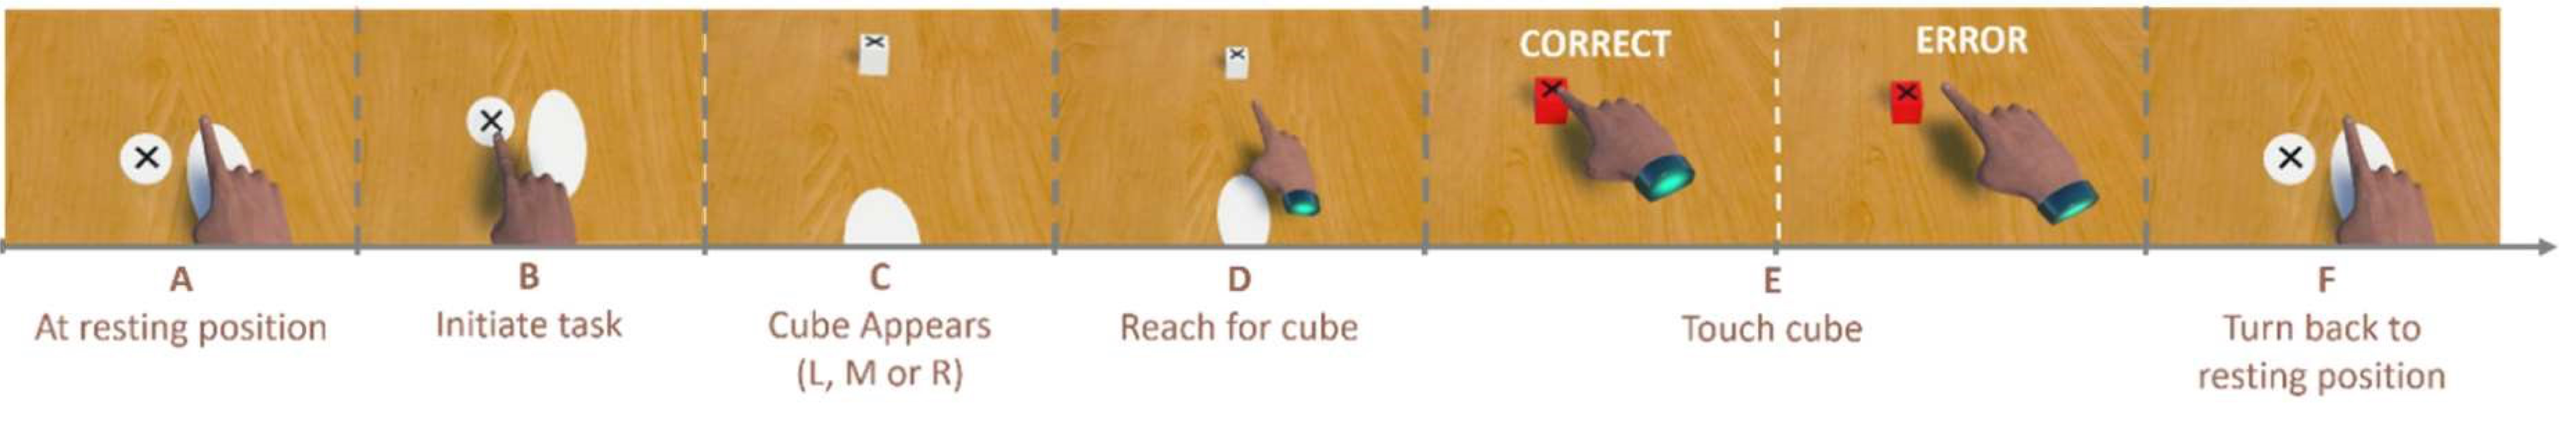
\includegraphics[width=\linewidth]{figures/task_setup.png}
\caption{The task.}
\end{figure}